\documentclass{ctexart}
\title{Algorithm Homework1}
\author{PB18111704 Zhu Enzuo}
\date{\today}
\usepackage{algorithm} %ctan.org\pkg\algorithms
\usepackage{algpseudocode}
\usepackage{amsmath}
\usepackage{tikz}
\begin{document}
\maketitle

\subsection{Prob1}
\paragraph{a1}线性查找伪代码如下
\begin{algorithm}
    \caption{线性查找}\label{euclid}
    \begin{algorithmic}[1]
    \Procedure{Fetch}{$A,v$}
    \For{$i\gets 1, n$}
        \If{$a_i=v$}
            \State \textbf{return} $i$
        \EndIf
    \EndFor
    \State \textbf{return} $NIL$
    \EndProcedure
    \end{algorithmic}
\end{algorithm}
\paragraph{a2}循环不变式证明如下
\subparagraph{初始化} 首先需要证明迭代开始之前循环不变式成立。此时i=0,已查找的元素集合中和v不相等的元素的集合S为$\emptyset$。而空集中不会有元素和v相等。
\subparagraph{保持} 我们需要证明每一次循环之后$v\notin S$,而我们可以看到只有满足$a_i\not= v$的$a_i$才会被加入到S当中。故该性质对循环成立。
\subparagraph{终止} 当循环中途跳出的时候,说明我们找到了一个$a_i=v$,满足要求。当循环正常结束之后,说明对任意$a_i$,都有$a_i\not=v$,满足题目要求。故我们可以得出结论该算法是正确的。

\paragraph{b}平均需要检查的元素个数$P=\sum_{k=1}^n \frac{k}{n} =\frac{k+1}{2}$,最坏情况需要检查的元素个数为n。$f(A,v)=O(n)=\Theta (n)$

\subsection{Prob2}
\paragraph{a} 错误。考虑$f(n)=\frac{1}{n}$,可以发现$O(f(n)^2)=\frac{1}{n^2}<f(n)$。
\paragraph{b} 正确。利用$\Theta$的定义,取$c1=1, c2=2, n_0=1$,有$\forall n\ge n_0, 0\leq max(f(n),g(n))\leq f(n)+g(n)\leq 2max(f(n),g(n))$。故命题正确。
\paragraph{c} 错误。取$f(n)=n,O(f(n))=n^2$,有$\Theta (f(n))=n$,显然$f(n)+O(f(n))=n^2\not= \Theta(f(n))$。
\paragraph{d} 错误。$f(n)=\Sigma (g(n)) \to \exists n_0, \forall n>n_0, f(n)\leq g(n)$,而后者与之矛盾。

\subsection{Prob3}
\paragraph{证明}$lg(n!)=\Theta(nlg(n))$
\begin{align*}
    n! &=\sqrt{2\pi n}(\frac{n}{e})^n e^{\alpha_n} \\
    lg(n!) &=lg(\sqrt{2\pi n})+nlg(n)-nlg(e)+\alpha_n lg(e) \\
           &=\Theta(lgn)+\Theta(nlgn)+\Theta(n)+\Theta(\frac{1}{n})\\
           &=\Theta(nlgn)
\end{align*}
\paragraph{证明}$n!=\omega(2^n)$\\
令$n_0=4$,则$\forall n\ge n_0$, 有\\
$n!=n*(n-1)*(n-2)*...*4*3*2*1 \ge 2*2*2*...*2*2*2*2$\\
故$n! = \omega(2^n)$\\
\paragraph{证明}$n!=o(n^n)$\\
令$n_0=2$,则$\forall n\ge n_0$,有\\
$n!=n*(n-1)*(n-2)*...*2*1 \leq n*n*n*...*n*n $\\
故$n! = o(2^n)$

\subsection{Prob4}
\paragraph{证明}假设$T(n)=O(lgn)$\\
不妨设T(n)=O(lgn),则对于$n_0=2$,有$2lg2 \ge T(2)=T(1)+1=2$\\
又$\forall n>n_0$,若已知$T(n)\le 2lgn$,有$T(n+1)=T(\frac{n+1}{2})+1 \le 2lg(\frac{n+1}{2})+1=2lg(n+1)-2lg2+1=2lg(n+1)-1 \le 2lg(n+1)$\\
故$T(n)=O(lgn)$

\subsection{Prob5}
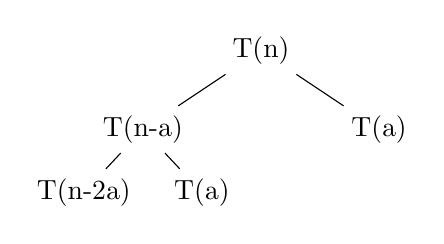
\begin{tikzpicture}[level distance=1.3cm,
        level 1/.style={sibling distance=3cm, level distance=1cm},
        level 2/.style={sibling distance=1.5cm, level distance=0.8cm}]
     \node {T(n)}
        child {node {T(n-a)}
            child {node {T(n-2a)}}
            child {node {T(a)}}
        }
        child {node {T(a)}
     };
\end{tikzpicture}
树的深度是$\left \lfloor \frac{n}{a} \right \rfloor$,第h层的值为c(n-ha)。故可求得
\begin{align*}
    O(T(n)) &=\sum_{h=0}^{\left \lfloor \frac{n}{a} \right \rfloor} c(n-ha) \\
            &=c\sum_{h=0}^{\left \lfloor \frac{n}{a} \right \rfloor} (n-ha) \\
            &=c\sum_{h=0}^{\left \lfloor \frac{n}{a} \right \rfloor}n - c\sum_{h=0}^{\left \lfloor \frac{n}{a} \right \rfloor}ha\\
            &=O(n^2)
\end{align*}

\subsection{Prob6}
\paragraph{a} $T(n)=\sqrt{n} lgn$
\paragraph{b} $T(n)=n^2$

\subsection{Prob7}可以,由于对于递归式有$n^{\log_2 4} < n^2lgn$,故其渐进界$O(T(n))=n^2lgn$
\end{document}
